\documentclass[USenglish]{article}

%\usepackage[utf8]{inputenc}%(only for the pdftex engine)
\RequirePackage[no-math]{fontspec}[2017/03/31]%(only for the luatex or the xetex engine)
\usepackage[small]{dgruyter}

\usepackage{natbib}
\bibliographystyle{apalike}

\usepackage{microtype}

\begin{document}

  \articletype{Research Article}

  \author*[1]{C.J.(Chaojie) Duan}
  %\author[2]{...}
  %\author[1]{...} 
  \runningauthor{Duan}
  \affil[1]{Dulun Consulting Group, research@dulun.com}
  %\affil[2]{...}
  \title{Latent vs. Observable Home-Field Advantage in Professional Soccer}
  \runningtitle{Bayesian Hierarchical Analysis}
  \subtitle{A Multilevel Bayesian Operationalization}
  \abstract{Home Field Advantage (HFA) was traditionally defined in terms of winning percentage of home games at the team level. In this article, we present a hierarchical model of HFA, spanning from the top sport level to the middle league level and all the way to lowest club level. Using scoring performance data from ESPN FC, we fit a Bayesian multilevel nested model to the parameters in the hierarchical model of HFA, allowing information obtained from the season level to inform the inferences about scoring rates at the upper team, league, and sport levels. Our analysis of latent HFA reveals that much of HFA is attributed to the nature of the sport of interest. While only a handful of teams out of 98 in top 5 European leagues enjoy statistically significant HFA, we found absolutely no teams suffer from home disadvantage.}
  \keywords{European Professional Soccer Leagues, Latent Home Field Advantage, Poisson generative process, Stan}
  %\classification[PACS]{...}
  %\communicated{...}
  %\dedication{...}
  \received{5/21/2018}
  %\accepted{...}
  \journalname{Journal of Quantitative Analysis in Sports}
  %\journalyear{...}
  %\journalvolume{..}
  %\journalissue{..}
  \startpage{1}
  %\aop
  %\DOI{...}
\maketitle

\section{Introduction} 

%The National Football League is tapping Amazon Web Services to help power its “Next Gen Stats” platform.
%Aiming to uncover deeper insights into the games of professional football, the National Football League (NFL) recently announced that it will be powering its Next Gen Stats with Amazon's Cloud Computing Platform - AWS to kick off the 2018 season. %with more impactful and meaningful content.  
%Amazon’s cloud computing arm also powers Statcast, the next generation statistics platform for Major League Baseball (MLB). These high-profile tech-sport partnerships are arguably the latest and most visible account of invasion of analytics into the realms of spectator sports.

In professional team sports, the term home field advantage (HFA) – also called home advantage, home ground or home court advantage, defender's advantage, home-ice advantage – describes the benefit that the home team is believed to gain over the visiting opponent. Its scientific definition is ``the consistent finding that home teams in sport competition win over 50\% of the games played under s balanced home and away schedule'' \citep[p. 13]{Courneya1992}.
Due to the existence of HFA, many vital games, such as playoff or elimination matches, in major professional sports have special rules for determining which match is played at which place.  As shown in Figure \ref{fig11}, the combined revenue of the Big Five European soccer leagues (English Premier League, Spanish La Liga, French Ligue 1, Bundesliga, Italian Serie A) more than doubled to 15 billion euros in 10 years from 2006/07 to 2016/17. The financial implications might partially explain UEFA's (the Union of European Football Associations) decision that a second leg of any Champions League knock-off series is favorable to playing away with the the scores still in balance after the first leg competition \citep{atkins2013}.

%----------------------
\begin{figure}[ht]
\caption{\textit{Revenue of the top European soccer leagues (Big Five*) from 2006/07 to 2016/17 (in billion euros)}}
\centering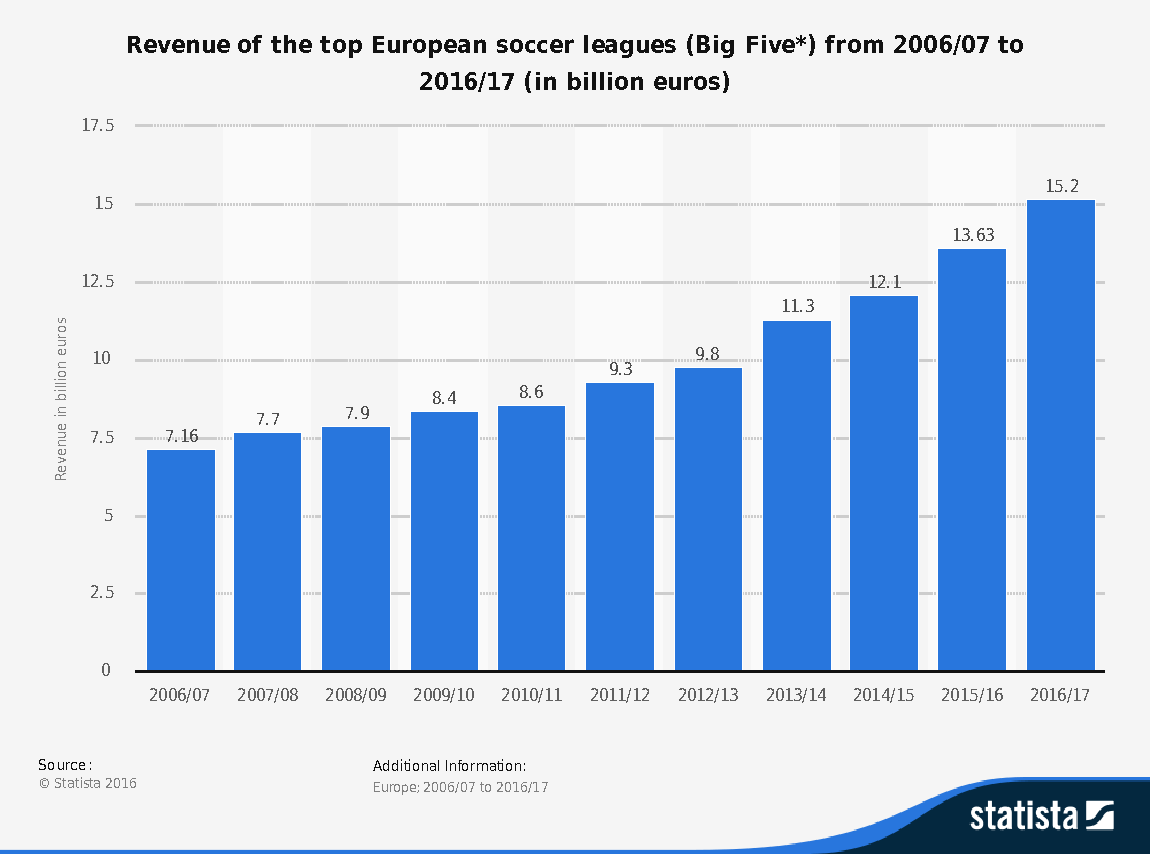
\includegraphics[width=0.8\textwidth]{HFA11.pdf}. 
\label{fig11}
\end{figure}
%------------------------

The existence of HWP (home winning percentage) -denominated HFA measure has been well documented for a variety of sports, even though the contributing factors are still being debated. In their book \textit{Scorecasting}, \cite{moskowitz2012scorecasting} compiled the HWPs in all the major sports with some datasets going back as further as 1903 for MLB and 1966 for NFL. MLS figures date back to only 2002, but show the strongest evidence of HWP of 69.1\%. MLB figures, on the other hand, yield the lowest HWP of only 53.9\%. This disparity raises an important high-profile question: ``Are all sports created equal in terms of HFA?''. A subsequent but related question is ``Is HFA primarily determined by the sport being played or teams who play the sport?''. Answering such questions demands a completely new way of conceptualizing HFA and signals a major departure from the reigning framework proposed by \cite{Courneya1992}, which hinges on game being the unit of analysis.  


%Accompanying the wide-spreading notoriety in the general populace is the ever-increasing availability and volume of data associated with games, players, teams, and sports.   

%a new platform that uses data from player and ball tracking devices to produce new advanced statistics like distance covered, speed, and acceleration — the idea is to better show a receiver’s ability to get open, for example, or how well the offensive line protects the quarterback. The information is shown to fans online and on TV broadcasts; teams also leverage the data internally for strategic purposes.

%we’ll be able to kick off our 2018 season with even more impactful and meaningful content, uncovering deeper insights into the game of football than we’ve ever done before,” 

%Matt Swensson, vice president of emerging products and technology at the NFL, said in a statement. “We chose AWS because of its combination of advanced cloud offering, powerful machine learning capabilities, and experience operating at the scale we need.”

 

%\citep{Gajewski2006}
%\citep{Carron2005}


A second motivator for this study is related to the treatment of sports data in general, and scoring in soccer matches in particular. HWP based measures tend to upstage and upgrade the originally discrete count-based outcome to continuous type, while ignoring the underlying data generating process. To complicate matters further, consider the two extreme cases of all winning and losing regular season. The HWP and AWP(away winning percentage) are equal, taking values of either 1.o or 0.0. If we adopt HWP as the sole indicator of HFA, we go straightforward to absurd conclusions - the all winning club enjoys 100\% HFA and the zero-win team suffers from 100\% home field disadvantage.   

The current conceptualization and operationalization of HFA prompt us to take an alternative route in search of true latent HFA underlying the numbers in record books. Specifically, we seek in this paper to achieve the following goals: 

\begin{enumerate}
\item  Propose a fresh new vertical hierarchical model of HFA, complementing the existing horizontal framework.
 

\item Highlight the different generative process underlying most sports performance metrics and suggest corresponding approaches for analysis.
\item Reveal sources of HFA simultaneously at sport, league, team levels.
\item Presenting a new way of measuring latent HFA via contrast the same performance metric at home and away venues. 
\end{enumerate}

The remainder of the paper is organized as 
 
\section{Review of Literature} 

\ref{fig21}

%------------------------------------------------
\begin{figure}
\caption{The Hierarchical Structure of Professional Soccer }
{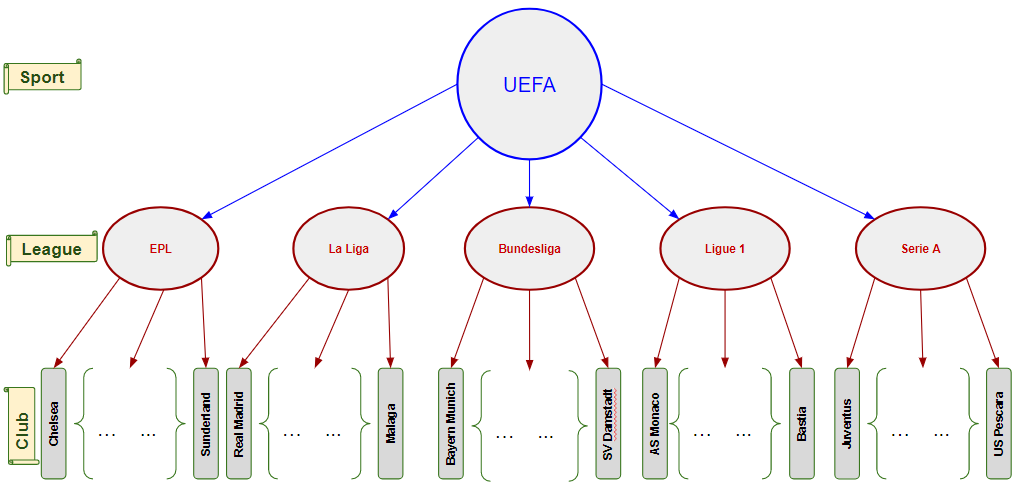
\includegraphics[width=1.0\linewidth]{HFA_22}}
\label{fig21}
\end{figure} 
%------------------------------------------------ 
 

\section{The Hierarchical Model of HFA} 

The essence of Bayesian inference is fitting a probability model to a dataset and generating probability distributions on the parameter encapsulated by the model \citep{Gelman2014}.
For our project, the data set contains the season (s) -level best home and away scoring numbers ($y^H_{ijs}$ and   $y^A_{ijs}$ respectively) of each club i in each j of the Top 5 leagues. As shown in figure \ref{fig33}, our hierarchical model reflects the organizational structure of professional soccer shown in figure \ref{fig21}.



%------------------------------------------------
\begin{figure}
\caption{The Hierarchical Model of Home Field Advantage }
{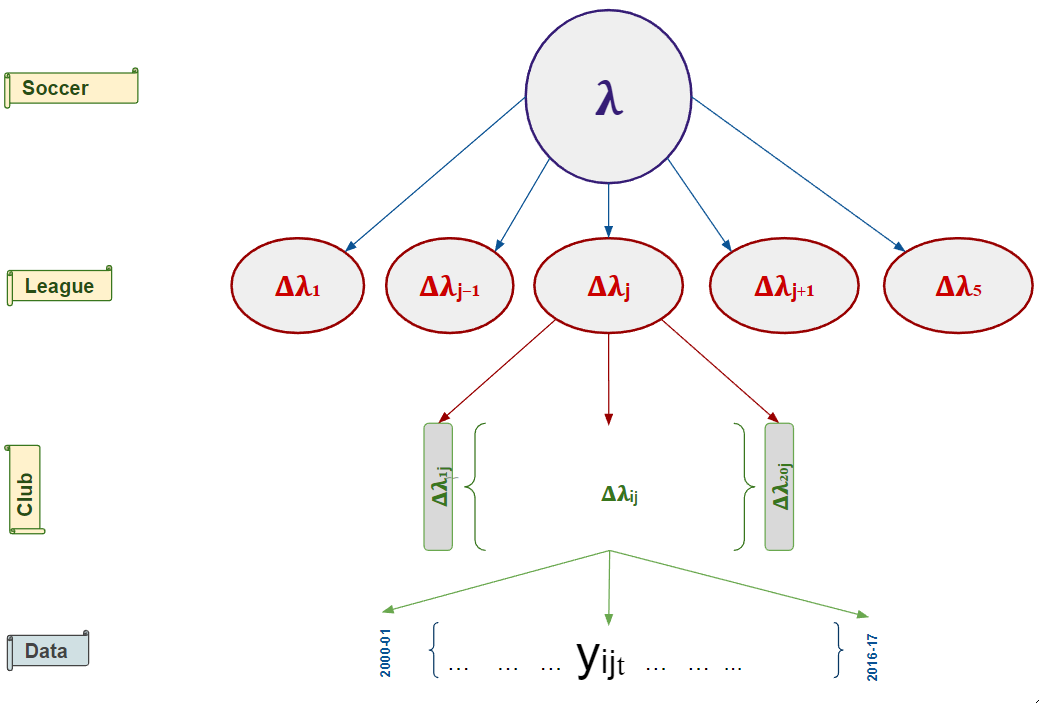
\includegraphics[width=1.0\linewidth]{HFA_33}}
\label{fig33}
\end{figure} 
%------------------------------------------------ 






\section{Data and Results} 



%-----------------------
\begin{table}[ht]
\caption{Descriptive Statistics}
\centering
\begin{tabular}{cccccccc}
\starttabularbody
\hline 
 & Mean & Median & Std. Dev. & Min. & Max. & Skewness & Kurtosis\\
\hline
 MHG & 3.634 & 4 & 1.676 & 0 & 9 & 0.246 & 0.034 \\
\hline 
 MAG & 2.884 & 3 & 1.676 & 0 & 10 & 0.627 & 0.786 \\
\hline
\end{tabular}
\label{tab1}
%{Goal Scoring Metrics: Most Home \& Away Goals at the Season Level} 
\end{table}
%=====================================================

We run 4 chains using the default sampler in Stan, the HMC variant of No-U-Turn Sampler (NUTS) \citep{Hoffman2014} and set  

The model estimates are shown in figure \ref{fig31} as shift from the 0. The outer contour lines show the 99.5\% credible intervals, while the shaded area underneath covers the corresponding 95\% credible interval. The light bar in the middle represents the mean.

\begin{figure}
\caption{Home Field Advantage Posterior Plot at Sport and League Levels}
{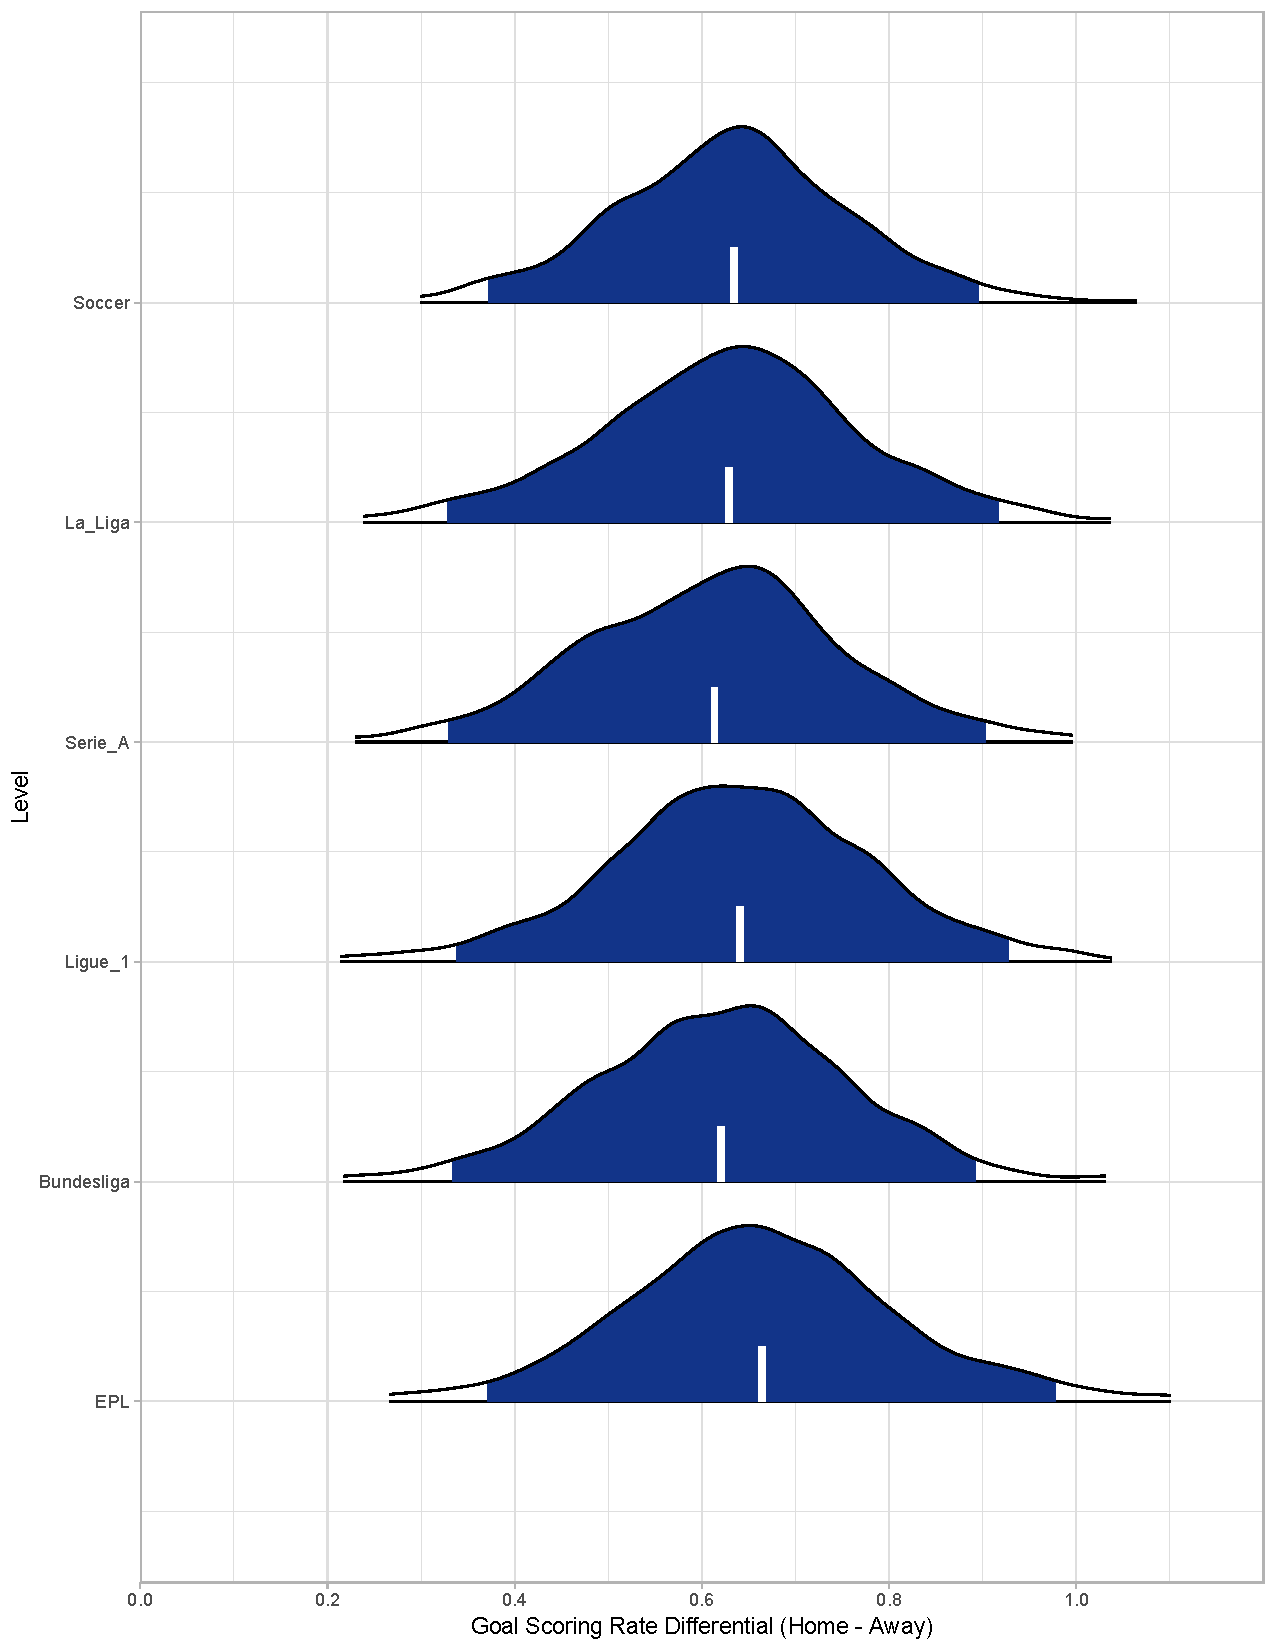
\includegraphics[width=0.80\linewidth]{HFA32.pdf}}
\label{fig31}
\end{figure}



\begin{figure}
\caption{Home Field Advantage Posterior Plot for La Liga Teams}
{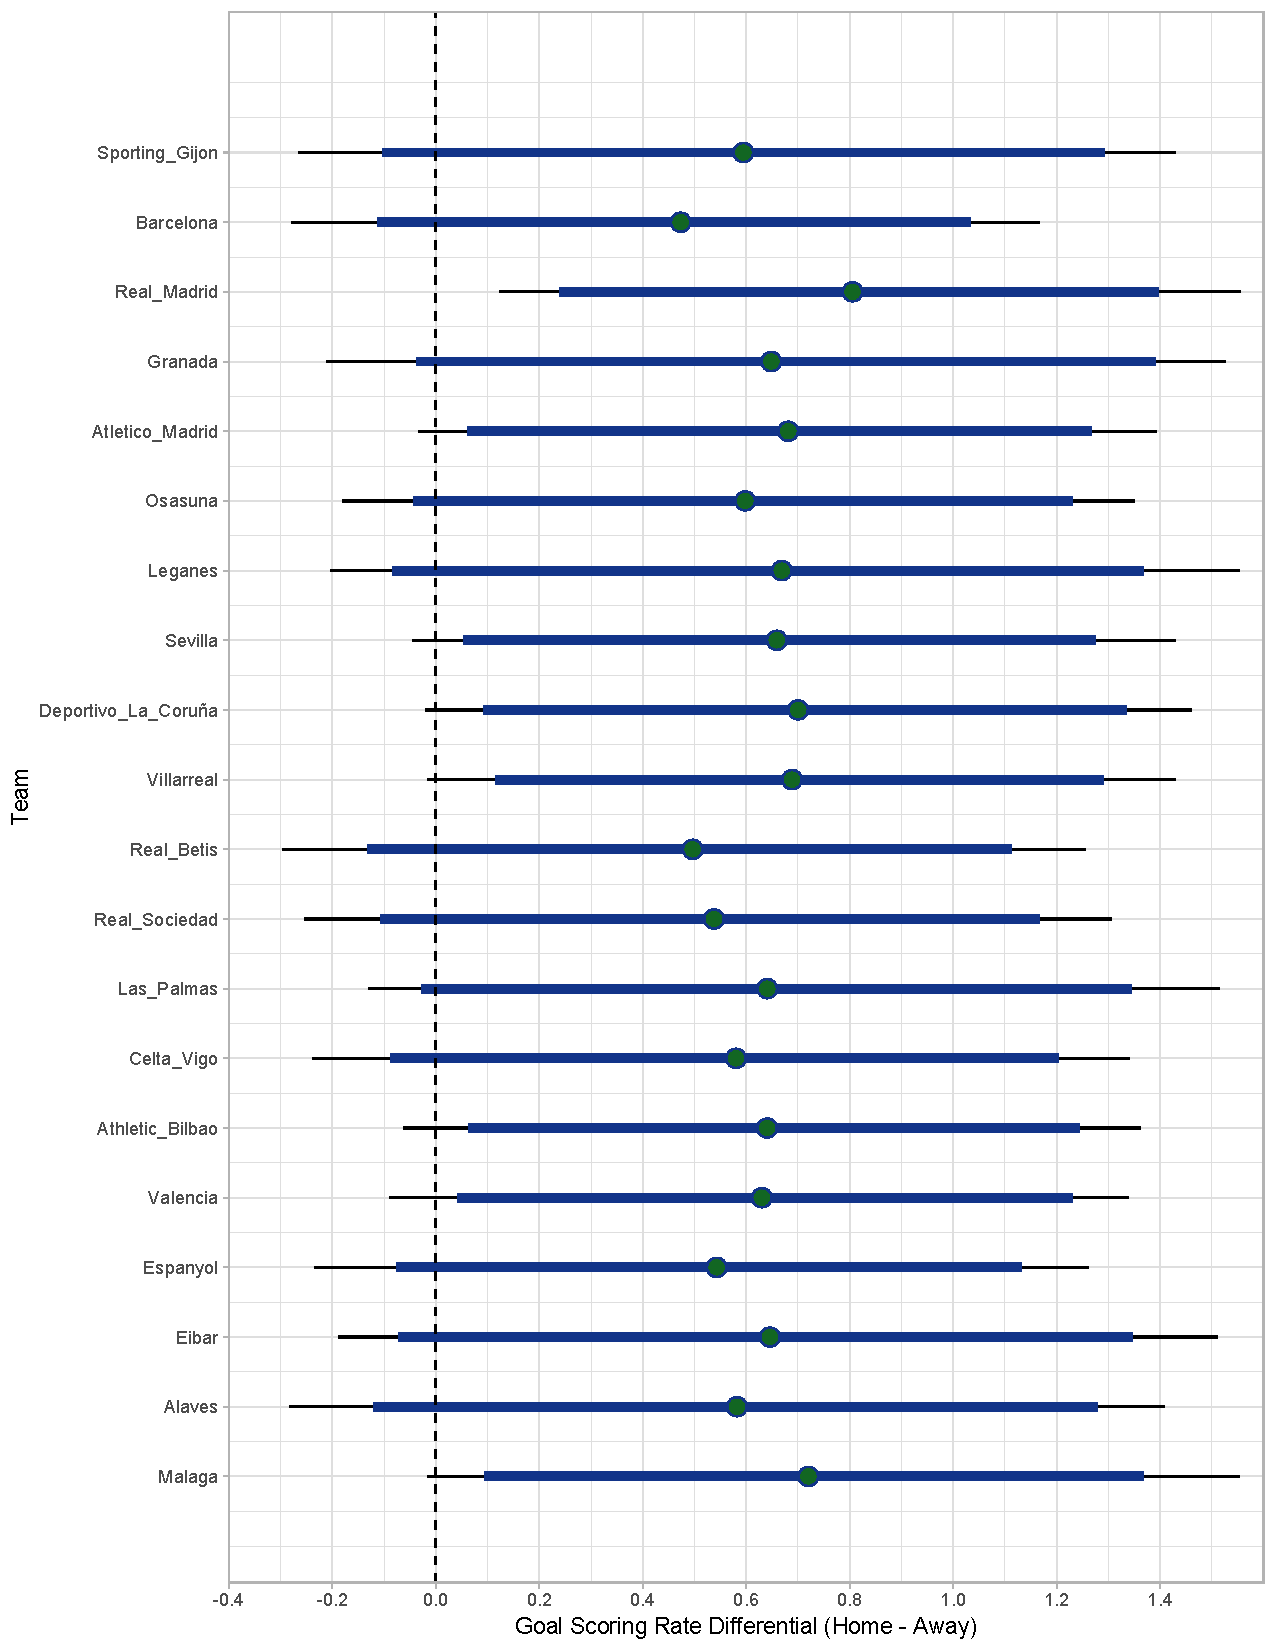
\includegraphics[width=0.90\linewidth]{HFA_La_Liga11.pdf}}
\label{fig32}
\end{figure}


\begin{figure}
\caption{Home Field Advantage Posterior Plot for Serie A Teams}
{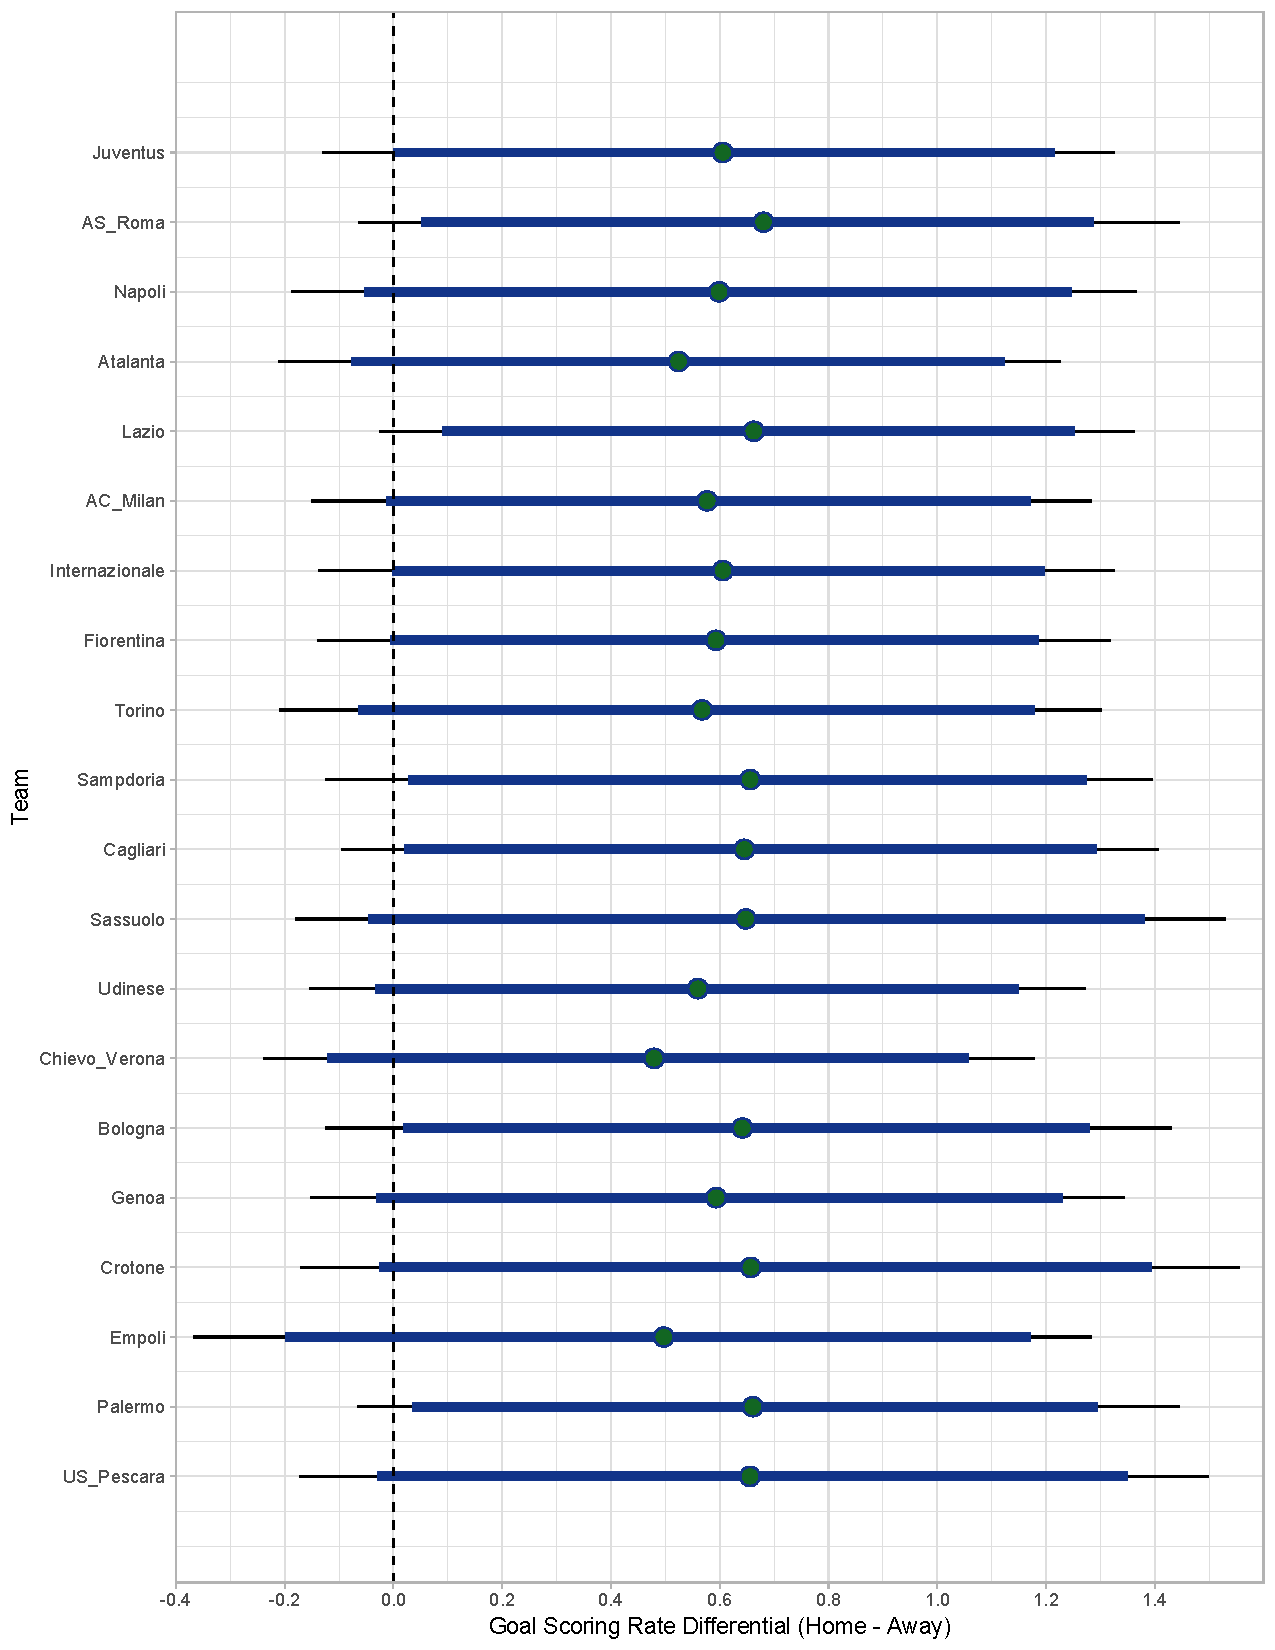
\includegraphics[width=0.90\linewidth]{HFA_Serie_A11.pdf}}
\label{fig4}
\end{figure}

\begin{figure}
\caption{Home Field Advantage Posterior Plot for Ligue 1 Teams}
{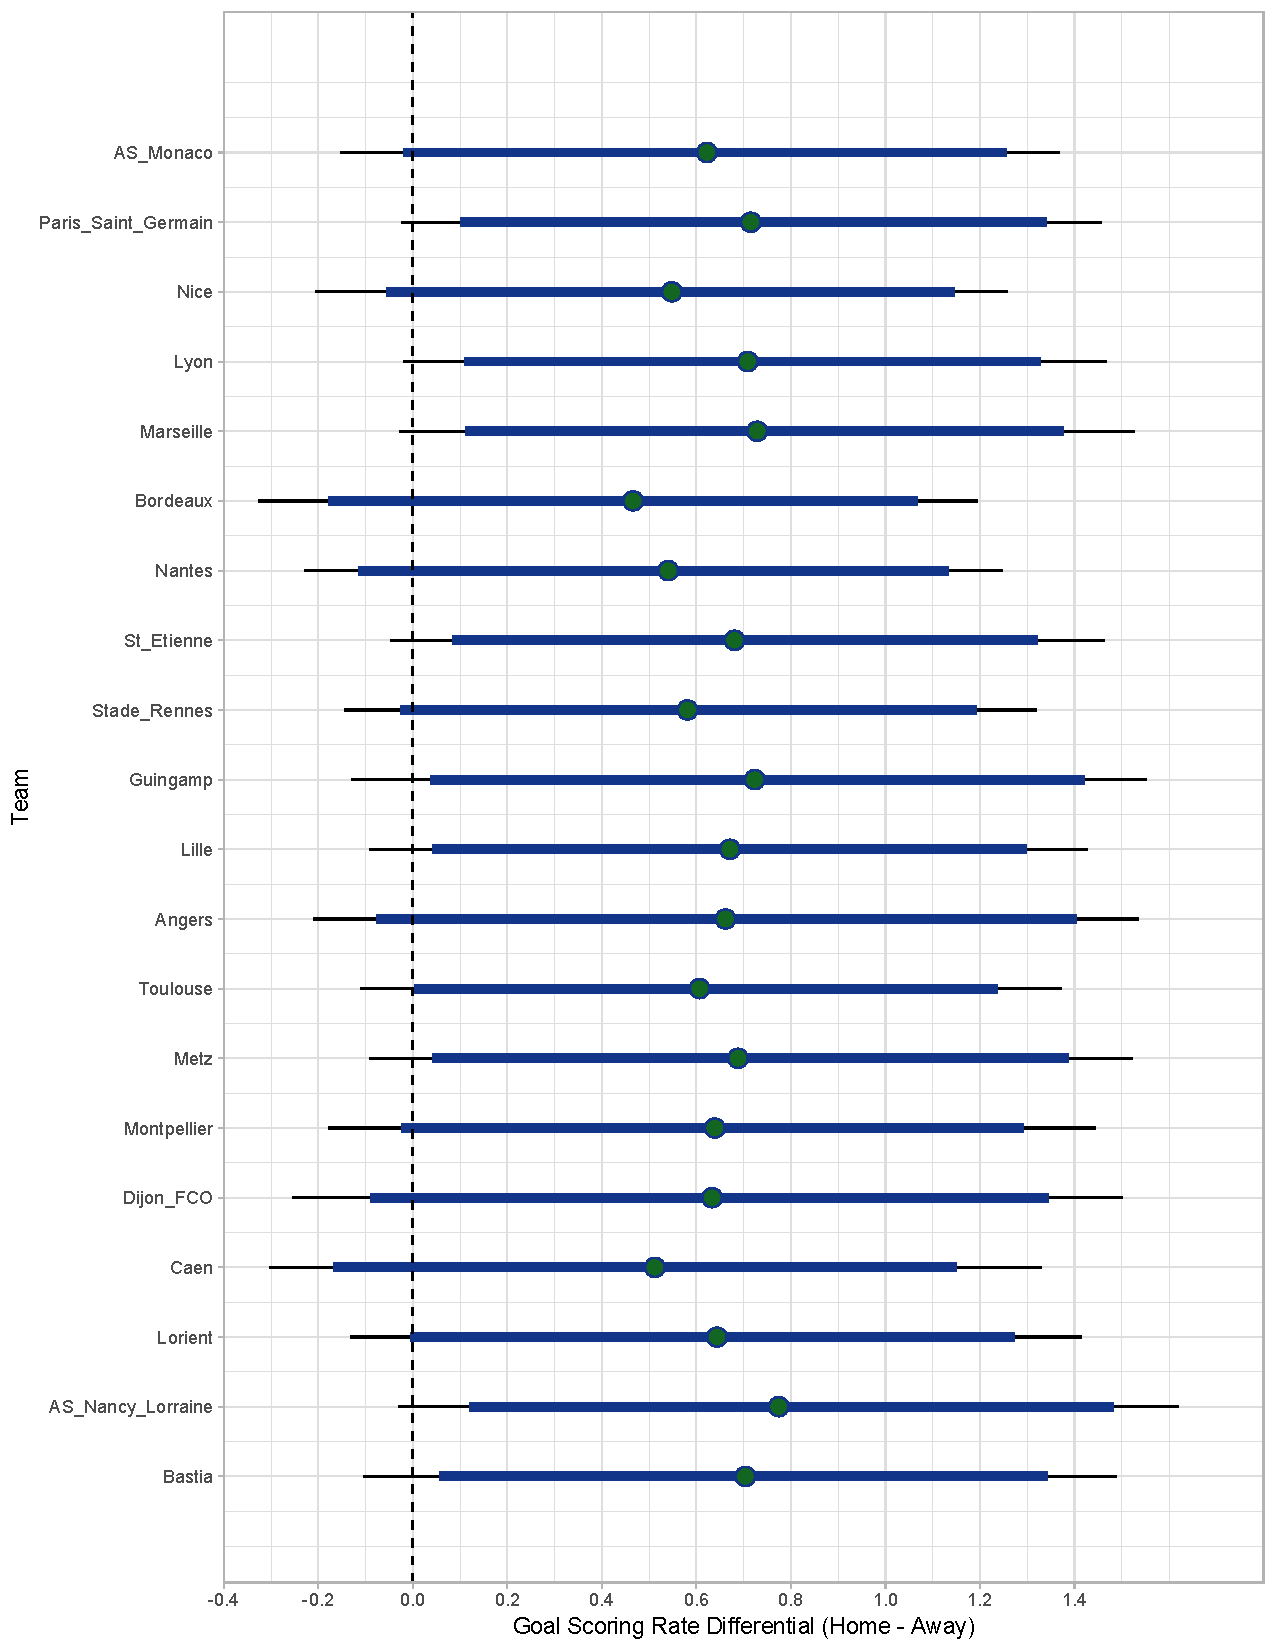
\includegraphics[width=0.90\linewidth]{HFA_Ligue111.pdf}}
\label{fig5}
\end{figure}

\begin{figure}
\caption{Home Field Advantage Posterior Plot for Bundesliga Teams}
{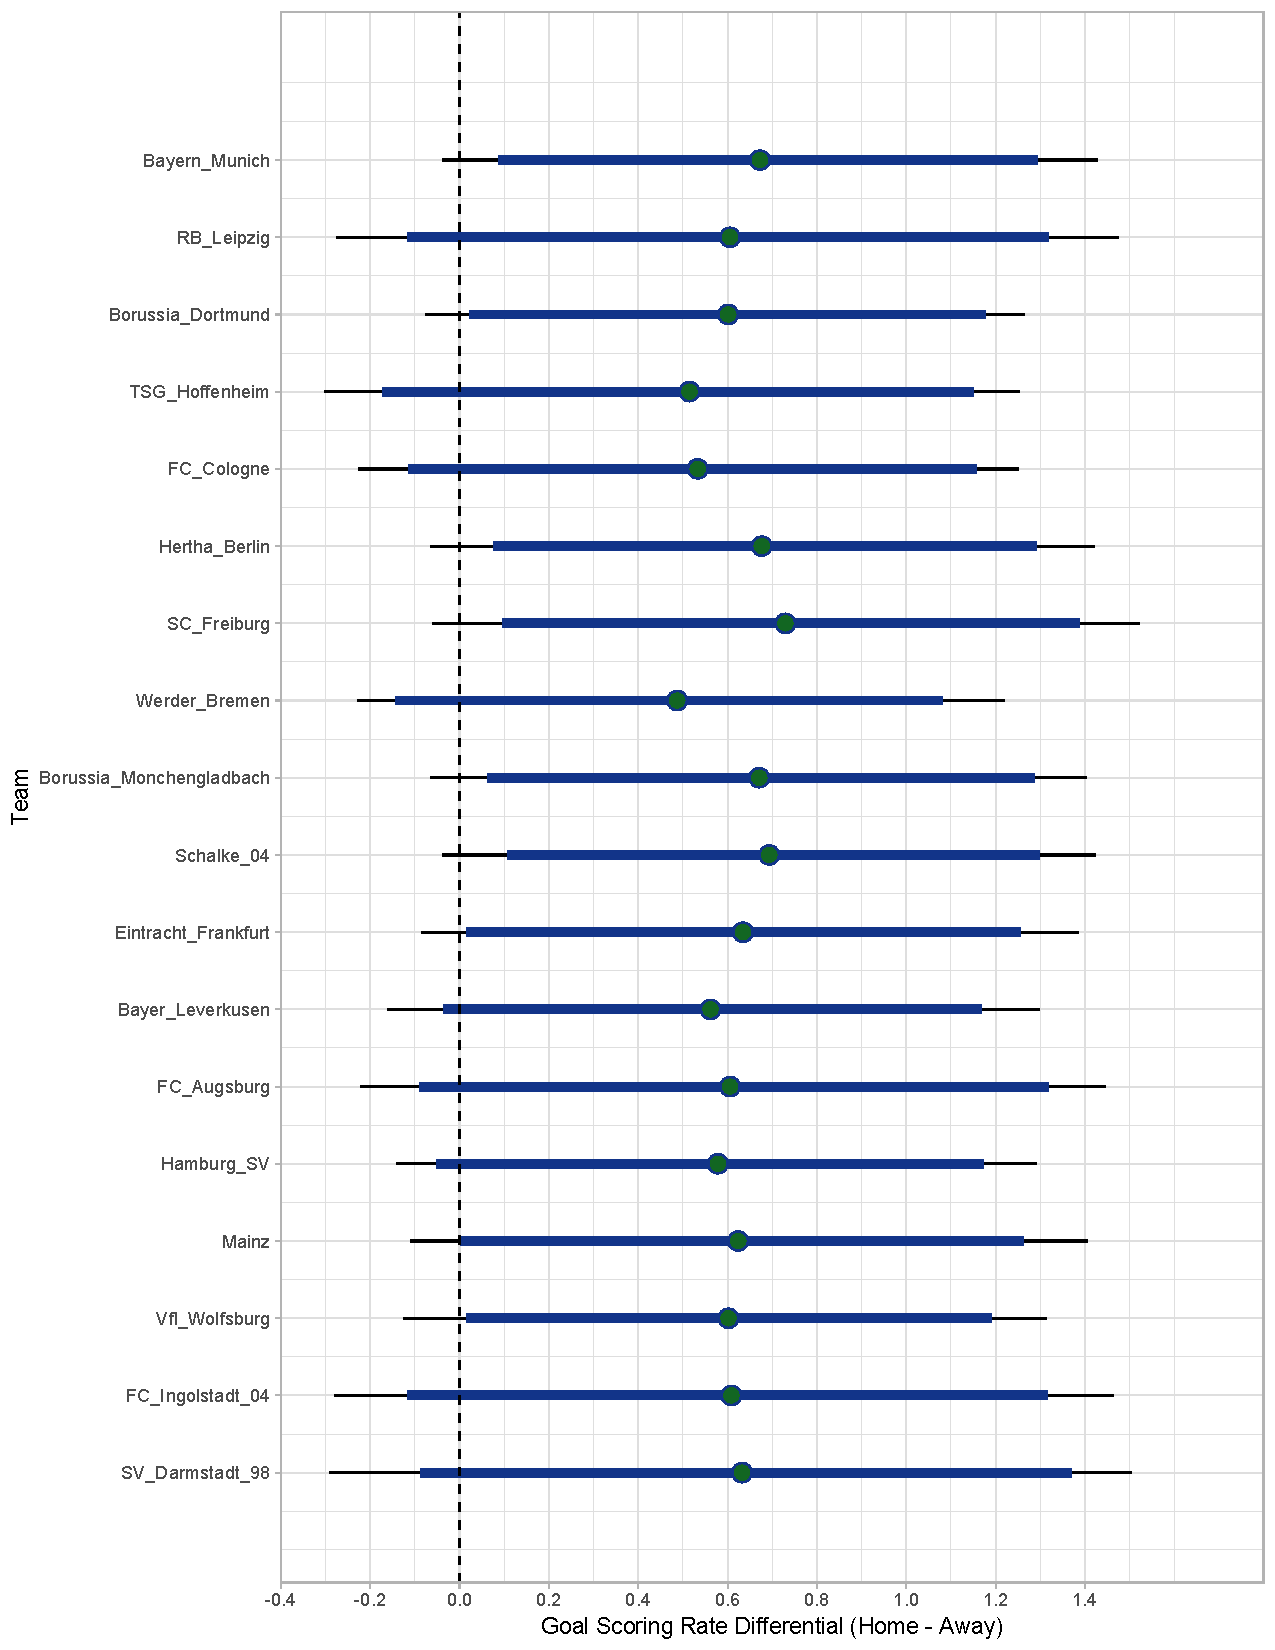
\includegraphics[width=0.90\linewidth]{HFA_Bundesliga11.pdf}}
\label{fig6}
\end{figure}

\begin{figure}
\caption{Home Field Advantage Posterior Plot for English Premier League Teams}
{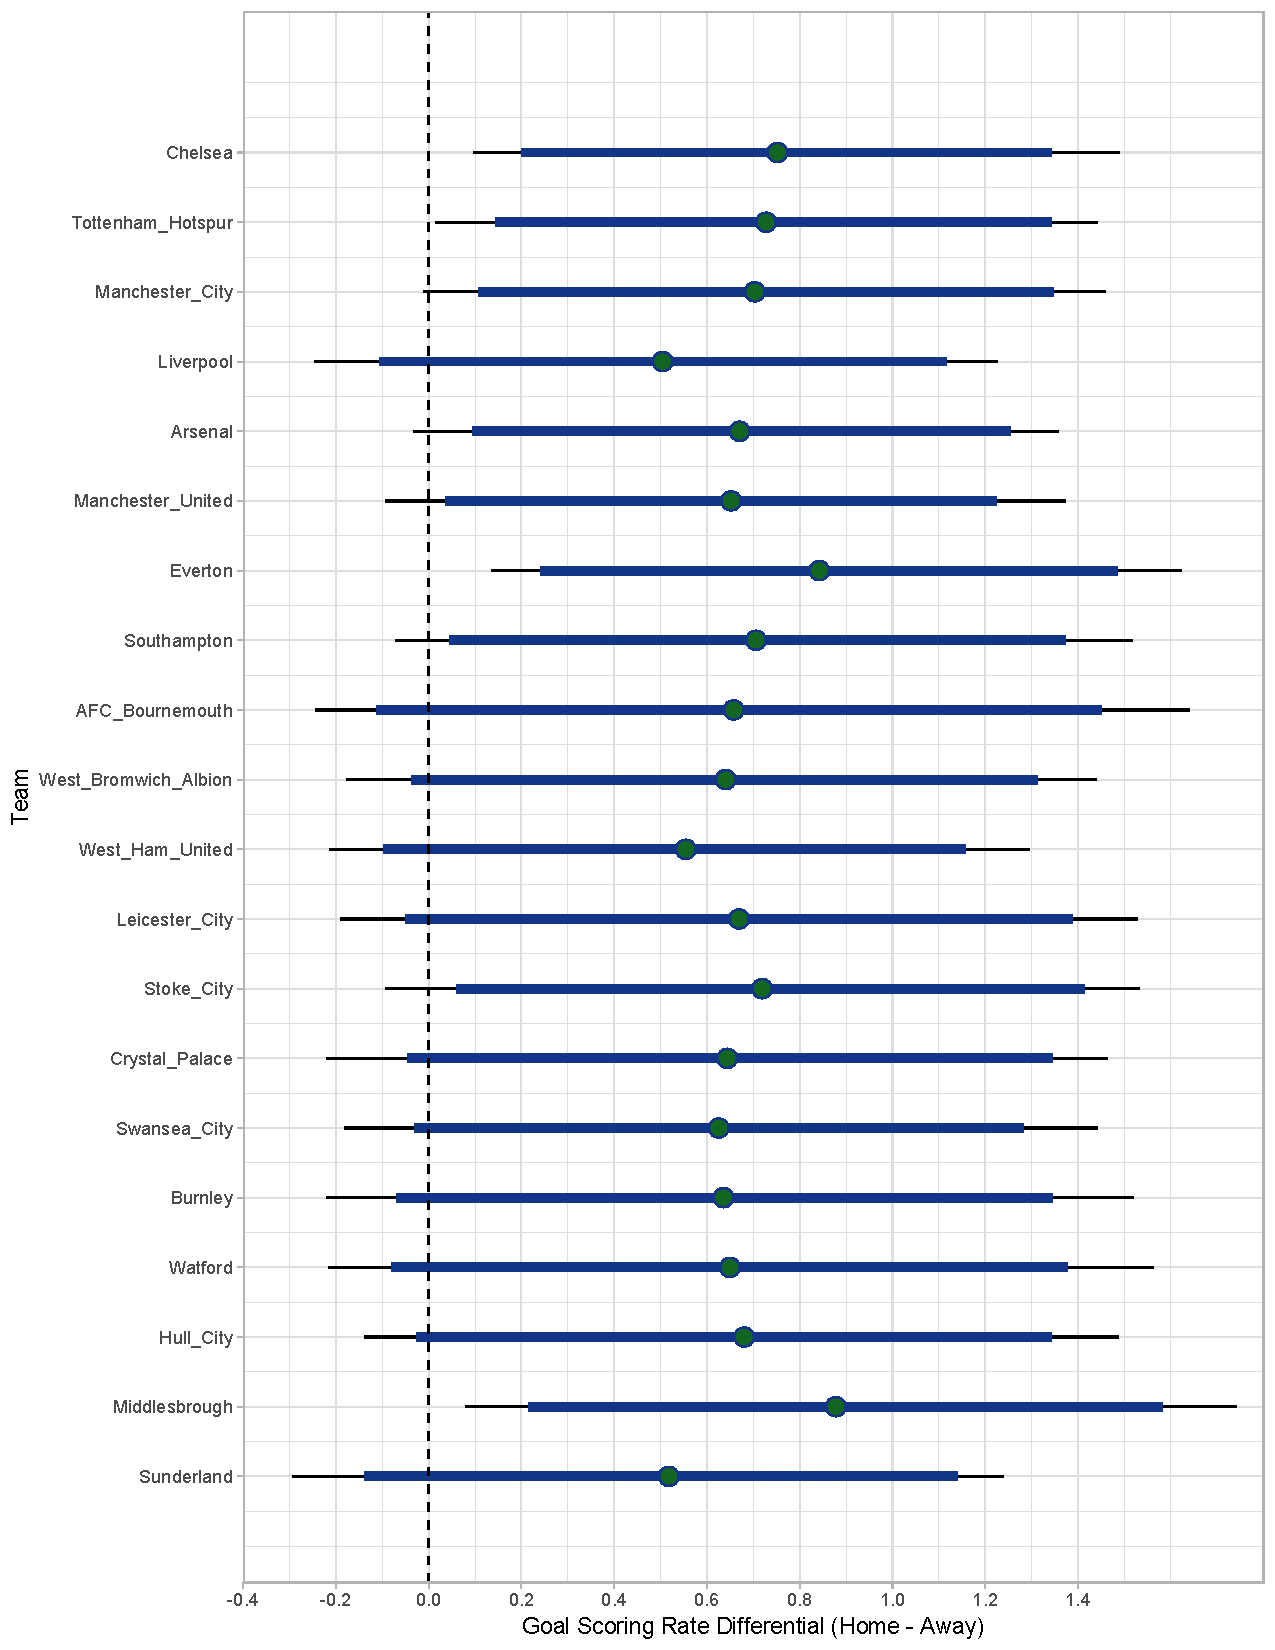
\includegraphics[width=0.90\linewidth]{HFA_EPL11.pdf}}
\label{fig7}
\end{figure}


\begin{acknowledgement}

We would like to thank ESPN FC for compiling the season-level club performance data and allow public access.

\end{acknowledgement}

\newpage

%\bibliographystyle{name}
\bibliography{Soccer,Bayesian}
\end{document}
